% 2016 공주대 워크숍
% 텍 매크로 작성법

\documentclass{beamer}

\usetheme{metropolis}
\metroset{inner/sectionpage=none}
\metroset{outer/progressbar=head}
\metroset{color/block=fill}
\usefonttheme[onlymath]{serif}

\usepackage{kotex}
\usepackage{mathtools}

\hypersetup{pdfencoding=auto}


% title
\title{텍 매크로 작성법}
\subtitle{텍 매크로 작성의 기초와 응용}
\author{남수진}
\date{2016년 11월 5일(토)}
\institute{
  2016 공주대학교 문서작성 워크숍 2016\\
  공주대학교 인문사회과학관 1층 컴퓨터실 107호}


%%
\begin{document}

\maketitle


%
\begin{frame}{매크로 관련 명령어}
  \vspace{4mm}
  \hbox to\hsize{\hss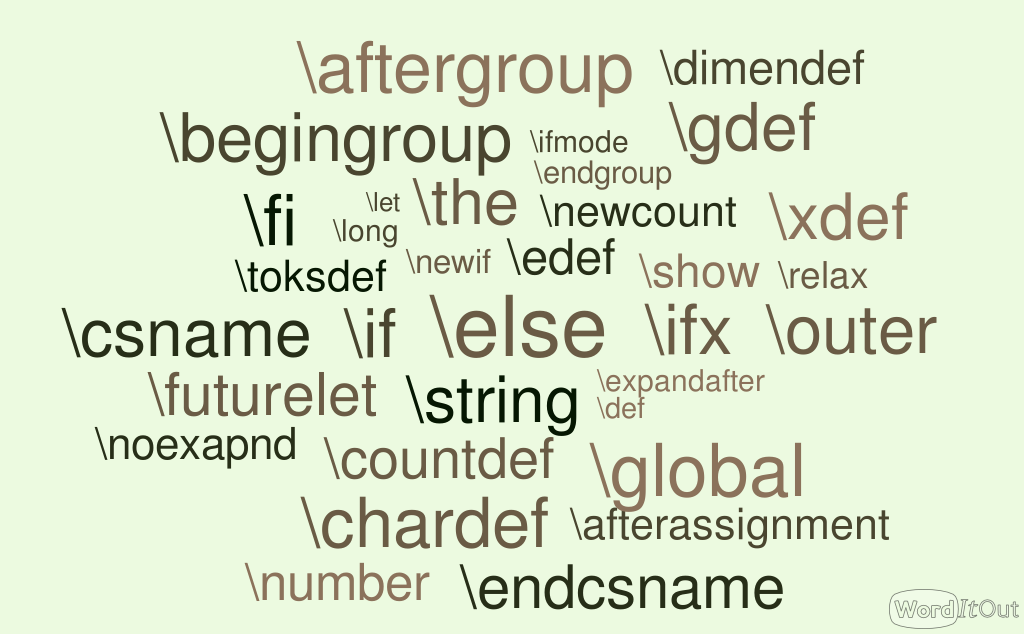
\includegraphics[height=7.5cm]{cs.png}\hss}
\end{frame}


%
\begin{frame}[fragile]{매크로 정의}
  \begin{itemize}
  \item 문서에서 여러번 반복적으로 사용되는 문구나 명령어의 나열을 하나의 명령어로 만든 것
    
    \medskip
    \hbox to\hsize{\hss
      \verb+\def+<control sequence><parameter text>%
      \verb+{+<replacement text>\verb+}+\hss}
    \medskip
  \item 텍의 전개 과정에서 매크로는 치환문으로 교체된다.
  \item 텍은 입력(input), 전개(expansion), 실행(execution), 출력(visual)의 과정을
    거친다.
  \end{itemize}
\end{frame}


%
\begin{frame}[fragile]{매크로}
  The \TeX\ Hierarchy, TUGboat, Volume 15 (1994), No.1, 7---9.
  \begin{description}
  \item [Novice] has heard of macros, but has never seen one.
  \item [User] writes macros that are used once, and that are
    longer than the code they replace.
  \item [Programmer], having been bitten by unwanted spaces,
    writes macros that don't contain spaces, and every line ends with
    a `{\small\verb+%+}'.
  \item [Hacker] has written self-modifying macros, writes
    {\small\verb+\endlinechar=-I+} or {\small\verb+\catcode'\^-M=9+}
    to prevent having to put {\small\verb+%+}'s at the end of lines in macros.
  \item [Guru] has written macros containing {\small\verb+####+}, more than 3
    {\small\verb+\expandafter+}'s in a row, and the sequence
    {\small\verb+\expandafter\endcsname+}.
  \end{description}
\end{frame}


%
\begin{frame}{오늘의 환율}
  \begin{center}
    \Large \href{http://fixer.io}{\texttt{Fixer.io}}\\
      {JSON API for foreign exchange rates and\\ 
        currency conversion}
  \end{center}
\end{frame}


%
\begin{frame}{발표자료}
  \begin{itemize}
  \item \url{https://github.com/sjnam/2016-kts}
  \item \url{https://github.com/sjnam/luagmp}
  \end{itemize}
\end{frame}


%
\plain{\huge ¿Tienes alguna pregunta?}


\end{document}

